\section{\texorpdfstring{\pony{Scale Out: From Individual Adaptation to Population-Scale Personalization}}{Scale Out: From Individual Adaptation to Population-Scale Personalization}}\label{sec:scale-out}

\begin{figure}[tbp]
    \centering
    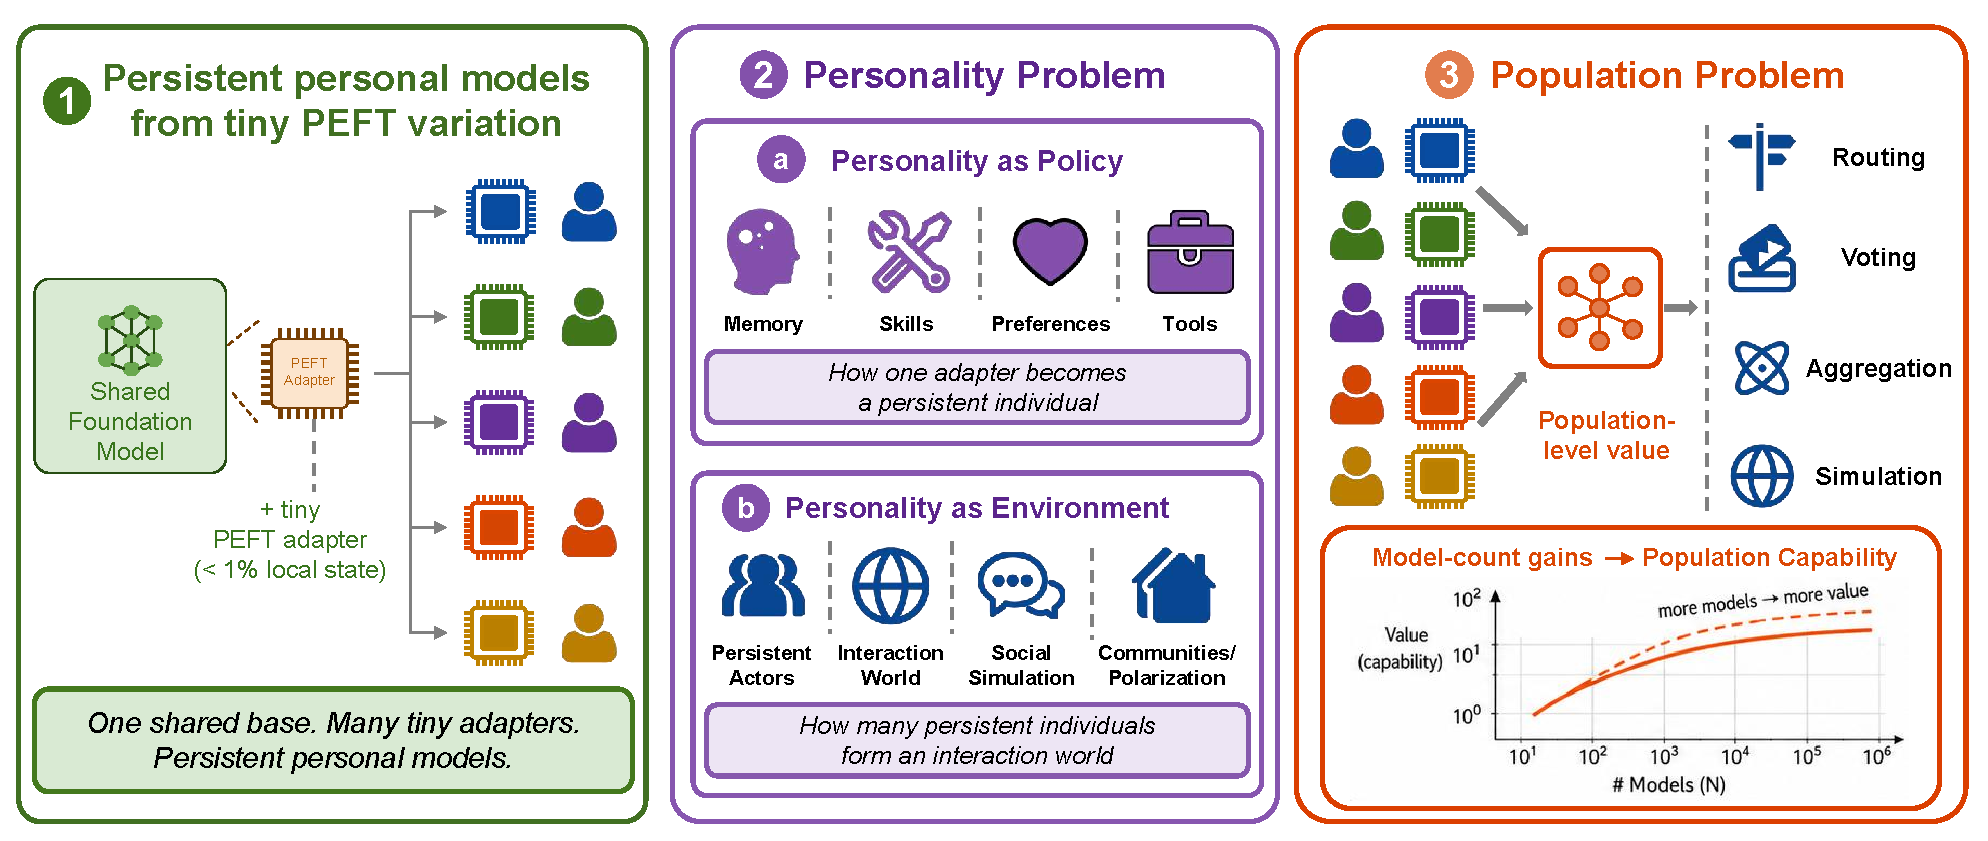
\includegraphics[width=\linewidth]{figures/scale_out/scale_out_teaser.pdf}
    \caption{\pony{Scale Out maps small stable variation to population-level value. A shared base model supports persistent personal models through lightweight PEFT adapters. Scale Out requires both preserved individuality and population-level utility.}}
    \label{fig:scale-out-teaser}
\end{figure}



\pony{Scale Down identified the operating regime in which the local adaptive state becomes small, stable, and cheap enough to be trained, stored, updated, and served repeatedly. Scale Out begins when such adaptation becomes routine. The question is no longer only how to improve one adapted model, but what becomes possible when many persistent personal model instances can exist at the same time. PEFT makes this question concrete: a shared foundation model can support many isolated adapters, each carrying a different local state.}

\pony{Adapter count alone, however, is not a scaling law. If many adapters collapse toward the same policy, model count is only redundancy. If adapters remain different but their differences cannot be simulated, composed, selected, or aggregated, diversity remains local personalization. Scale Out therefore asks three connected questions, each addressed by a subsection below: (1) how personal models preserve continuity for individuals, including what to memorize, how to write memory into adapter parameters, and how to govern learned capabilities (Section~\ref{subsec:personality-adapters}); (2) how persistent user-conditioned policies can support user simulators and agent environments (Section~\ref{subsubsec:personality-as-environment}); and (3) how diversity among adapted models can become a source of collective performance (Section~\ref{subsec:population-capability}).}

\pony{A note on Context Learning: it appears in Section~\ref{subsec:personality-adapters} as the \emph{write policy} for LoRA-as-memory, the mechanism that decides which context-time improvements should be stabilized into adapter parameters. It is not a standalone Scale Out algorithm. Its role is to make memory-signal efficiency tractable: without a principled write policy, LoRA memory capacity is a hard ceiling, but with one, repeated interaction can selectively fill that capacity with behaviorally useful state.}

\subsection{\pony{Personal Models for Individuals}}\label{subsec:personality-adapters}

\pony{A personal model is not just a universal assistant with a longer prompt. It needs persistent adaptive state, so that repeated experience can shape future behavior. A task adapter can be disposable: it solves a benchmark or domain and can be replaced when the task changes. A personal adapter instead carries part of the enduring state for one user, agent, role, or workflow: memories, preferences, skills, and tool habits. The adapter stores part of the learned behavioral state, not the entire user history.}

\pony{Personal adaptation has two roles in Scale Out. As a user-conditioned policy, it explains how a shared base model becomes a persistent personal model for one user. As a simulated environment component (\Cref{subsubsec:personality-as-environment}), it explains how many such persistent policies can form user simulators or agent environments. The final population subsection then asks a separate question: whether differences among adapted models can be aggregated into measurable system-level performance.}


\paragraph{From adapter to personal policy.}
\pony{The first function of local adaptive state is policy specialization. A personal model should not merely answer in a preferred tone. It should help decide what to remember, which tools to prefer, how to ask questions, when to avoid action, how to recover from failures, and which behaviors are natural or unacceptable for a particular user. In this sense, personalization is not decoration. It is the policy layer that determines how a shared base model becomes useful for one person. Adapter isolation turns personalization from a global update problem into a local policy problem: the base model remains shared, while experience and behavior become user-specific. The rest of this subsection develops this view in four steps: memory is a precondition for continuity, memory requires a capacity law, bounded capacity requires a write policy, and once adapters shape tools and skills, personalization becomes an agentic capability.}

\paragraph{Memory as the precondition of personality.} 
Personality requires memory because a model cannot remain itself without preserving experience across interactions. Preferences, habits, past failures, recurring tasks, relationships, and learned workflows all depend on accumulated state. Prompt-based personalization is transient; retrieval-based memory is external and must be reinterpreted at every turn; parametric memory offers the stronger possibility that selected experience becomes part of the model's own policy. This motivates the LoRA-as-memory question: can a lightweight adapter serve as a bounded memory substrate for personal state? Since conversational and agent memory require more than recognition accuracy \citep{packer2024memgpt,chhikara2025mem0,maharana2024longmemory}, a personal adapter must support recall, addressing, reasoning, overwrite, conflict resolution, and behavioral application.



\paragraph{LoRA as memory: capacity scaling law.}
To support millions of personal models, we need scaling laws linking adapter size to capacity, stability, and retrieval accuracy. Key questions include how capacity correlates with LoRA rank, target modules, training tokens, and base-model scale, and when storage becomes detrimental interference.

% 这一段其实是介绍我们提出了报菜名的benchmark，如果太长可以放到附录
% Central to establishing these laws is a robust evaluation standard. A useful LoRA memory benchmark should cover four dimensions. (1) \textbf{Content coverage} asks whether facts, events, preferences, constraints, and procedures have been included. (2) \textbf{Structural coverage} asks whether temporal order, hierarchy, causality, and cross-segment dependencies are represented. (3)\textbf{ Difficulty coverage} asks whether tasks include direct recall, multi-hop reasoning, comparison, overwrite, and conflict resolution. (4) \textbf{Distributional coverage} asks whether generated queries resemble the downstream questions that the personal model will actually face. A benchmark that only converts context into convenient QA can overstate memory while missing the behaviors needed for personal models. We therefore introduce DishNameBenchmark as a controlled benchmark for isolating the core operations of LoRA memory. Although the surface task is simple, the abstraction is intentionally general: a dish name is a memory slot, a list of dishes is a local write, multiple turns create a sequential memory stream, a position query tests addressing, an adjacency query tests local relation, and a correction tests overwrite. This design lets us vary memory length, update frequency, query type, and correction pattern while keeping the underlying memory object interpretable. 

Establishing such laws requires a benchmark that measures more than convenient context-to-QA conversion. A useful LoRA memory benchmark should test content, structure, difficulty, and downstream query distribution, including recall, addressing, relation, overwrite, and conflict resolution. We therefore introduce DishNameBenchmark as a controlled benchmark for isolating core LoRA-memory operations. It abstracts memory into interpretable slot-writing and slot-querying tasks, allowing us to vary memory length, update frequency, query type, and correction pattern while keeping the stored object simple and measurable.


\begin{figure}[tbp]
    \centering
    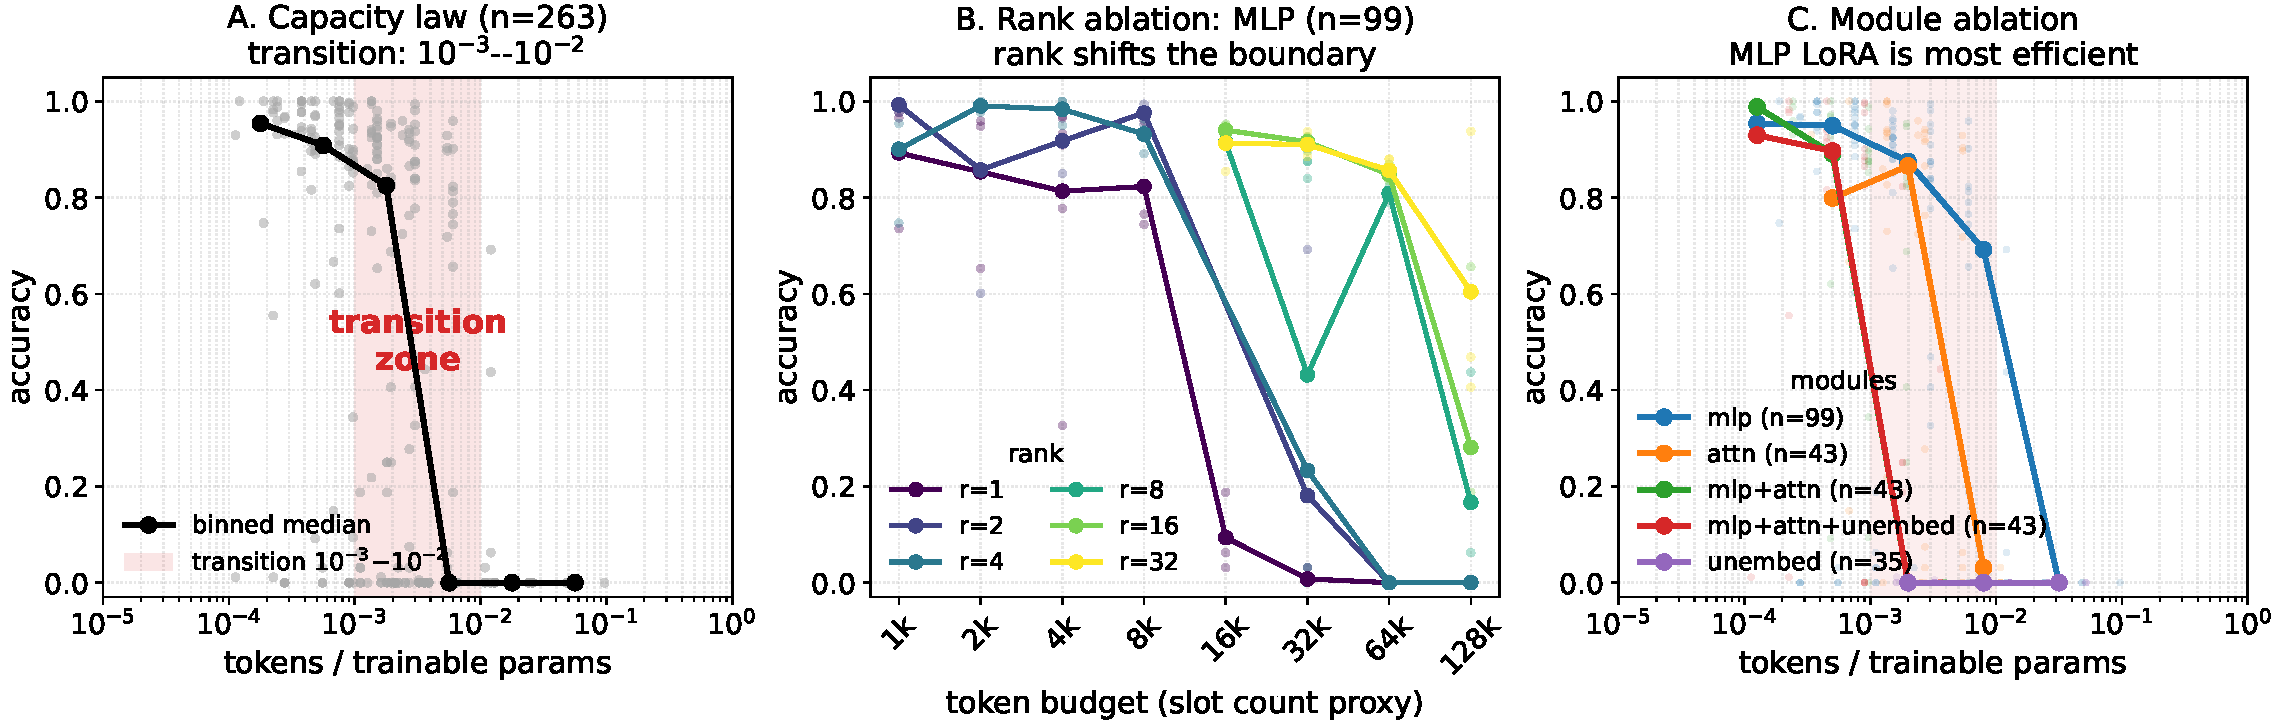
\includegraphics[width=\linewidth]{figures/scale_out/lora-as-memory-scaling-law.pdf}
    \caption{DishNameBenchmark reveals a bounded LoRA memory law: usable capacity lies around $10^{-3}-10^{-2}$ tokens per trainable parameter, degrades predictably after saturation, and is most parameter-efficient when memory is written into MLP LoRA.}
    \label{fig:lora-as-memory-scaling-law}
\end{figure}

We evaluate LoRA memory capacity on DishNameBenchmark using Qwen3-series models. We report capacity efficiency as the ratio between memory tokens and trainable parameters, and measure whether the model can correctly recover the stored slot values under position, adjacency, and correction-style queries. The results are shown in \Cref{fig:lora-as-memory-scaling-law}: 

\begin{itemize}
    \item The first result is \textbf{a sharp capacity transition}. Across 263 runs, accuracy stays close to one when capacity efficiency is below roughly \(10^{-3}\), begins to degrade in the transition region between \(10^{-3}\) and \(10^{-2}\), and collapses toward zero once the memory load exceeds about \(10^{-2}\) tokens per trainable parameter. This suggests that LoRA memory has a measurable capacity ceiling: \textbf{the empirical upper limit in this setting lies between \(10^{-3}\) and \(10^{-2}\) memory tokens per trainable parameter.}
    \item For a fixed parameter budget, \textbf{performance drops approximately linearly after the adapter reaches its capacity limit.} In the rank ablation, increasing the token budget initially preserves near-perfect accuracy, but once the memory load crosses the adapter's effective capacity, accuracy falls rapidly as the number of required slots increases. Rank mainly shifts the capacity boundary by increasing the number of trainable parameters. At low memory budgets, even small-rank adapters can match larger-rank adapters. At high memory budgets, larger ranks survive longer because they provide more total storage surface. This supports the interpretation that rank buys capacity, but does not remove the underlying capacity law.
    \item The third result concerns where memory should be written. In the module ablation, training MLP LoRA provides the best parameter efficiency. At matched parameter budgets, MLP adapters maintain high accuracy at larger capacity-efficiency values than attention-only adapters, combined MLP+attention adapters, or unembedding adapters. Attention-only and full-module training can store memory, but they are less efficient per trainable parameter. Unembedding-only training performs worst and collapses quickly. The observed ordering is approximately
    \[
    \mathrm{MLP} > \mathrm{Attention} \approx \mathrm{All} \gg \mathrm{Unembed}.
    \]
    From a scale-out perspective, this matters because personal adapters must be cheap to train, store, and serve. If the goal is to maximize memory capacity per parameter, \textbf{the most efficient design in this benchmark is to train MLP LoRA only}.
\end{itemize}

% 从scaling law说明，容量是由上限的，不能什么都记住，所以引入到下一章节，哪些需要被记住
These results make LoRA memory a scarce resource rather than an unlimited store. Diversity therefore cannot be produced by writing everything into every adapter. If usable capacity is bounded and module choice strongly affects parameter efficiency, the next question is not only how much a personal adapter can memorize, but what kind of information deserves to become stable local variation.

\paragraph{What to memorize: behavioral state, not raw facts.}
The next question is what deserves LoRA memory. Because LoRA memory is harder to inspect and more expensive to edit, it should not function as a general fact store. A personal model instead needs a memory hierarchy (\Cref{tab:memory-hierarchy}): editable facts should remain in retrieval, inspectable external reality should remain in tools, and LoRA should be reserved for persistent behavioral adaptation.

\begin{table}[tbp]
\centering
\small
\setlength{\tabcolsep}{6pt}
\renewcommand{\arraystretch}{1.20}
\caption{A practical personal model should decide which memory layer should store each kind of state.}
\label{tab:memory-hierarchy}
\fittowidth{%
\begin{tabular}{@{}M{2.8cm}M{4.2cm}M{6.2cm}@{}}
\toprule
\apphead Memory layer & Example & Best suited for \\
\midrule
\appkey{Context}          & Current conversation              & Short-term reasoning and local task state \\
\addlinespace[2pt]
\appkey{Retrieval memory} & Notes, documents, user facts      & Editable factual recall and large evidence stores \\
\addlinespace[2pt]
\appkey{Tool state}       & Calendars, files, databases       & External reality that should remain inspectable \\
\addlinespace[2pt]
\appkey{LoRA memory}      & Skills, habits, policy, persona   & Persistent behavioral adaptation \\
\bottomrule
\end{tabular}%
}
\end{table}

This hierarchy clarifies the role of LoRA memory. A rare document should stay in retrieval, a calendar event should remain tool state, and a recurring workflow should become skill memory. The memories that matter for Scale Out are not isolated facts, but behavior-shaping structures that make one adapted model reliably different from another. Skills are the natural target because they are reusable, procedural, and policy-shaping. Following the intuition of SKILL-0 \citep{skill02026}, the scale-out implication is that a personal adapter should become a compact library of learned behavioral state: workflows, tool-use habits, reasoning templates, domain heuristics, safety routines, and action policies.

\begin{figure}[t]
\centering
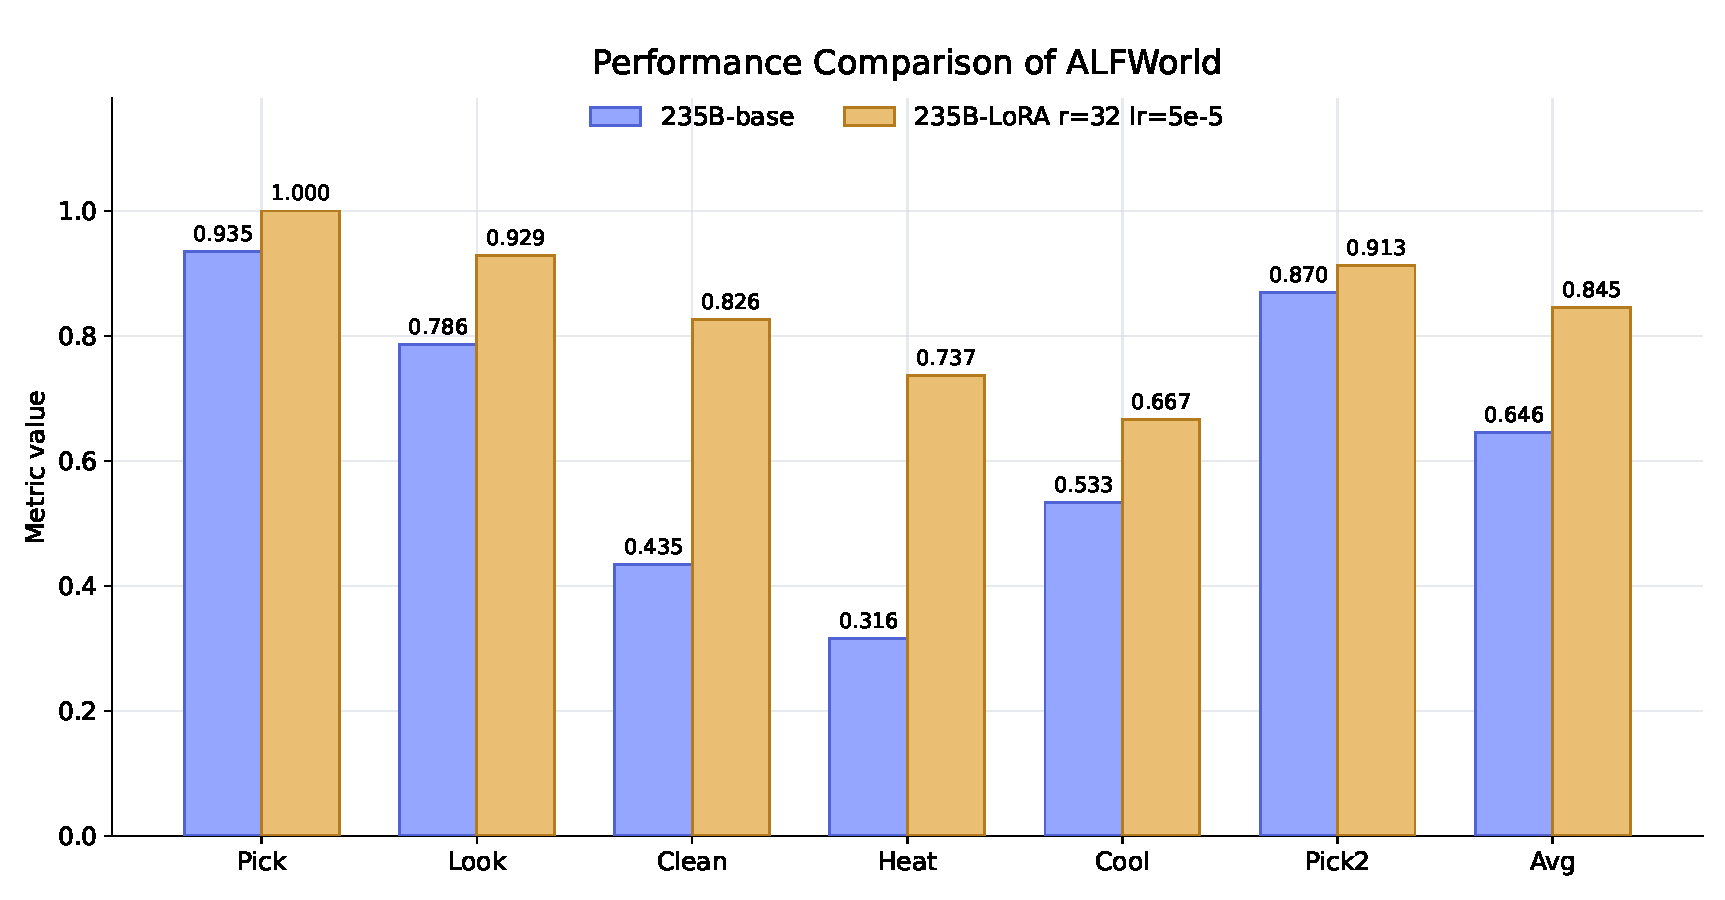
\includegraphics[width=0.80\textwidth]{figures/scale_out/skill0_alfworld_235b_lora_metrics.pdf}
\caption{LoRA skill memory on ALFWorld. Starting from Qwen3-235B, a rank-32 LoRA adapter trained with the Skill-0/MinT recipe improves ALFWorld validation performance over the base model across task categories, raising the average score from \(0.646\) to \(0.845\).}
\label{fig:skill0-alfworld-lora}
\end{figure}

We test this skill-memory interpretation by applying LoRA to a large-prior agent setting. Using Qwen3-235B as the shared base model, we train a rank-32 LoRA adapter with the Skill-0/MinT ALFWorld recipe and evaluate it on the ALFWorld benchmark. As shown in \Cref{fig:skill0-alfworld-lora}, the adapted model improves over the base model on all reported task categories, with the average metric increasing from \(0.646\) to \(0.845\). This result is not evidence that LoRA should store arbitrary facts. Rather, it supports the narrower claim that LoRA can store reusable skill-like behavioral state: the adapter changes how the model acts in a procedural environment.

% \textcolor{blue}{
% We will reproduce this line of evidence with LoRA: skill demonstrations will be encoded into adapters and compared against prompt-only, retrieval-only, LoRA-skill, and LoRA-plus-retrieval systems. The expected comparison is not whether an adapter can memorize a string, but whether it improves success rate, consistency, tool-use correctness, and generalization when a skill must be applied repeatedly.
% }


\paragraph{How to memorize: Context Learning as write policy.}
% 说完改记住什么东西以后，说一下如何记住这些信息
The memory hierarchy specifies where different states should live; Context Learning specifies how experience moves between layers. If Scale Down makes local variation cheap to store, Context Learning decides which temporary experiences should be stabilized into that variation. Context Engineering selects, retrieves, and arranges information to improve the current response. Context Learning asks which parts of that context-time improvement should become durable model state. In this sense, it is not merely better prompting, but the write policy of the personal model: it decides when repeated usefulness justifies converting context, retrieval, tool outcomes, or demonstrations into adapter parameters.

\begin{lstlisting}[
  language=Python,
  float=tbp,
  caption={Context Distillation as an on-policy context-to-parameters transfer. Context Learning as repeated Context Distillation.},
  label={lst:context-distill},
  basicstyle=\ttfamily\footnotesize,
  keywordstyle=\color{blue!70!black}\bfseries,
  commentstyle=\color{gray!70!black}\itshape,
  stringstyle=\color{green!45!black},
  numbers=left,
  numberstyle=\tiny\color{gray},
  numbersep=6pt,
  frame=single,
  rulecolor=\color{gray!35},
  backgroundcolor=\color{gray!6},
  xleftmargin=2.4em,
  xrightmargin=0.5em,
  framexleftmargin=2.0em,
  breaklines=true,
  breakatwhitespace=true,
  tabsize=4,
  showstringspaces=false,
  columns=fullflexible,
  keepspaces=true,
]
def context_distill(model, query, build_context, rl_update):
    # Step 1: query-only produces an on-policy rollout.
    out = model.sample(query)

    # Step 2: query + context scores the rollout.
    ctx = build_context(query)
    r_tok = model.token_reward(query, ctx, out)

    # Step 3: update from the query-only rollout and rewards.
    return rl_update(model, query, out, r_tok)

def context_learning(model, queries, build_context, rl_update, steps):
    for _ in range(steps):
        query = next(queries)
        model = context_distill(model, query, build_context, rl_update)
    return model
\end{lstlisting}

% 介绍一下context distillation是如何实现的
The mechanism begins with Context Distillation, summarized in \Cref{lst:context-distill} and \Cref{fig:context-distillation}. A query-only policy first produces an on-policy rollout. A stronger query-plus-context system then evaluates that rollout using retrieved evidence, demonstrations, tool outputs, execution outcomes, or slower verification. The resulting token-level or trajectory-level signal drives an RL-style update. Crucially, the update is applied to the query-only rollout, so the model learns to perform better without requiring the same context to be present at inference time. This differs from off-policy context distillation, where targets are produced with context and then learned without context through supervised fine-tuning \citep{snell2022distillingcontext}. Here, context is not used as a supervised target source; it is used as privileged information for scoring an output already produced by the query-only policy.

% 介绍一下context learning是如何实现的
Repeating this operation turns Context Distillation into Context Learning. At step \(t\), policy \(\pi_t\) answers a query without privileged context; the context system retrieves evidence, runs tools, observes outcomes, or performs slower verification; and the adapter is updated from this signal to produce \(\pi_{t+1}\). Future query-only behavior now starts from a stronger internal state. Related self-distillation methods also use additional information to create stable parameter updates \citep{hubotter2026selfdistillation,shenfeld2026continualselfdistillation}. Here, however, the loop is explicitly personalized: each iteration decides what part of a user's context, tools, outcomes, or demonstrations should become adaptive state.


% \begin{figure}[tbp]
% \centering
% \includegraphics[width=0.8\textwidth]{figures/scale_out/figure_06.png}
% \caption{Context Distillation updates the query-only policy using a query-plus-context teacher signal.}\label{fig:context-distillation}
% \end{figure}
\begin{figure}[tbp]
\centering
\resizebox{0.96\textwidth}{!}{\begin{tikzpicture}[x=1cm,y=1cm,>=Latex,line cap=round,line join=round,font=\footnotesize\sffamily]
  \tikzset{
    panel/.style={draw=mindlabfg, very thick, rounded corners=1.4mm, fill=white},
    softpanel/.style={draw=mindlabfg, very thick, rounded corners=1.4mm, fill=mindlabblue!10},
    stage/.style={draw=mindlabfg, very thick, rounded corners=1.4mm, fill=white},
    box/.style={
      draw=mindlabfg, thick, rounded corners=0.8mm, fill=white, align=center,
      inner sep=2pt, minimum width=1.55cm, minimum height=0.55cm,
      font=\footnotesize\sffamily
    },
    boxblue/.style={box, fill=mindlabbluepale!55},
    boxaccent/.style={box, fill=mindlabblue!22},
    boxsoft/.style={box, fill=mindlabfg!7},
    op/.style={
      draw=mindlabfg, thick, rounded corners=0.8mm, fill=mindlabblue!16, align=center,
      inner sep=2pt, minimum width=1.60cm, minimum height=1.30cm,
      text width=1.45cm, font=\footnotesize\sffamily
    },
    bigarrow/.style={->, line width=0.9pt, draw=mindlabfg, shorten >=2pt, shorten <=2pt},
    softarrow/.style={->, semithick, draw=mindlabfg!55, dashed, shorten >=2pt, shorten <=2pt},
    flowarrow/.style={->, line width=0.9pt, draw=mindlabfg, shorten >=3pt, shorten <=3pt},
    title/.style={font=\bfseries\footnotesize\sffamily, text=mindlabfg, align=center, fill=white, inner sep=2pt},
    stagetitle/.style={font=\bfseries\footnotesize\sffamily, text=mindlabfg, align=center, fill=white, inner sep=2pt},
    figtitle/.style={font=\bfseries\small\sffamily, text=mindlabfg, align=center},
    elabel/.style={font=\scriptsize\sffamily, text=mindlabfg, align=center, fill=white, inner sep=1.2pt},
    plainlabel/.style={font=\scriptsize\sffamily, text=mindlabfg!72, align=center, inner sep=0pt}
  }

  \path[use as bounding box] (-0.20,-3.45) rectangle (16.20,3.50);
  \node[figtitle] at (8.00,3.10) {Context Distillation: writing context gains into parameters};

  % Stage panels share top y = 2.20 and bottom y = -2.10
  % Column anchors (panel centers):
  %   S1 x=2.20  S2 x=6.55  S3 x=11.30  R x=14.95
  \def\Stop{2.20}
  \def\Sbot{-2.10}

  \node[stage] (s1) at (2.20,0.05)  [minimum width=3.30cm, minimum height=4.30cm] {};
  \node[stage] (s2) at (6.55,0.05)  [minimum width=4.20cm, minimum height=4.30cm] {};
  \node[stage] (s3) at (11.30,0.05) [minimum width=4.20cm, minimum height=4.30cm] {};
  \node[stage] (sR) at (14.95,0.05) [minimum width=1.70cm, minimum height=4.30cm] {};

  \node[stagetitle] at (2.20,2.05)  {Step 1\\Query-only rollout};
  \node[stagetitle] at (6.55,2.05)  {Step 2\\Context scoring \& rewards};
  \node[stagetitle] at (11.30,2.05) {Step 3\\RL-style parameter update};
  \node[stagetitle] at (14.95,2.05) {Result};

  % Stage 1 internals: aligned column at x=2.20, rows y=0.85,-0.10,-1.05
  \node[boxaccent] (q1)    at (2.20,0.85)  {Query};
  \node[boxblue]   (th1)   at (2.20,-0.10) {$\theta_t$};
  \node[boxsoft]   (out1)  at (2.20,-1.05) {Output};
  \draw[flowarrow] (q1.south) -- (th1.north);
  \draw[flowarrow] (th1.south) -- (out1.north);

  % Stage 2: inputs column x=5.45, op column x=7.65
  \node[boxaccent] (q2)   at (5.45,0.85)  {Query};
  \node[boxblue]   (ctx2) at (5.45,-0.10) {Context};
  \node[boxsoft]   (out2) at (5.45,-1.05) {Output};
  \node[op]        (rm)   at (7.65,-0.10) {Reward /\\scoring\\function};
  \draw[flowarrow] (q2.east)  -- (q2.east -| rm.west);
  \draw[flowarrow] (ctx2.east) -- (rm.west);
  \draw[flowarrow] (out2.east) -- (out2.east -| rm.west);

  % Stage 3: inputs column x=10.20, op column x=12.40
  \node[boxaccent] (q3)   at (10.20,0.85)  {Query};
  \node[boxblue]   (th3)  at (10.20,-0.10) {$\theta_t$};
  \node[boxsoft]   (rew3) at (10.20,-1.05) {$\{r_i\}$};
  \node[op]        (opt)  at (12.40,-0.10) {Optimizer /\\update\\function};
  \draw[flowarrow] (q3.east)  -- (q3.east -| opt.west);
  \draw[flowarrow] (th3.east) -- (opt.west);
  \draw[flowarrow] (rew3.east) -- (rew3.east -| opt.west);

  % Result
  \node[boxaccent] (thN) at (14.95,-0.10) [minimum width=1.30cm] {$\theta_{t+1}$};
  \node[plainlabel] at (14.95,-1.00) {distilled\\knowledge};

  % Stage-to-stage arrows (horizontal, between panels)
  \draw[bigarrow] (s1.east) -- (s2.west);
  \draw[bigarrow] (s2.east) -- (s3.west);
  \draw[bigarrow] (s3.east) -- (sR.west);

  % Carry-over: only one curve, from reward fn down/over to {r_i} input of stage 3.
  \draw[softarrow] (rm.south) .. controls (7.65,-2.85) and (10.20,-2.85) .. (rew3.south);
  \node[elabel, text=mindlabfg!75] at (8.92,-2.95) {token rewards $\{r_1,\dots,r_n\}$};
\end{tikzpicture}
}
\caption{Context Distillation updates the query-only policy using a query-plus-context teacher signal.}\label{fig:context-distillation}
\end{figure}

% 介绍RAG2LoRA为一个例子
RAG2LoRA illustrates this memory-layer transfer. The point is not that all retrieved facts should become parameters, but that retrieval can provide a teacher signal when it repeatedly improves behavior. Over time, recurring facts, preferences, and procedures can be partially internalized into the adapter, reducing dependence on perfect retrieval while leaving editable evidence in external memory. This is the memory-signal efficiency required for Scale Out: each user can maintain a personal adapter whose value grows with interaction while the base model remains shared.

\paragraph{Agentic personal models.}
The write-policy problem becomes most concrete in agentic systems, where the memory being written is often a workflow, tool habit, or post-failure correction. In this setting, the adapter is no longer only improving text generation; it is shaping how the model acts over files, messages, calendars, documents, code, tools, and long-running workflows. Personality becomes operational when memory determines continuity, skills determine competence, and policy determines safe action. This is where diversity begins to produce activity: different memories and skills lead agents to choose different tools, recover from different failures, and follow different workflows under the same external task. Related agent-learning work also treats skills and reflection as reusable learning objects \citep{shinn2023reflexion,xia2026skillrl}.

MindClaw \citep{li2026mindclaw} illustrates this transition from prompt-space skill growth to parametric skill consolidation. Textual skill libraries are useful during cold start, but over time they create skill drift and retrieval dependence: the library grows, prompts get longer, and the agent may still fail to trigger the right capability. The scale-out goal is therefore not a larger skill library, but a higher probability that useful skills are learned, triggered, and applied consistently.


% OpenClaw-style systems provide the natural substrate for this transition because they expose the model to persistent tools, user-specific workflows, and long-horizon interaction. However, much of their growth initially happens in the prompt space. Skills are generated and stored as text; memory is recovered by retrieving text back into context. This works during cold start, but it accumulates noise over time: generated skills can be vague, redundant, unused, or plausible only because a stronger model wrote them, and the deployed model may use them only when retrieval and prompt layout happen to be correct.

% MindClaw \citep{li2026mindclaw} treats personal OpenClaw as a parametric-memory problem. The agent layer uses MetaClaw for online conversation collection, skill injection, post-failure skill evolution, and RL sample collection. The infrastructure layer uses MinT to turn live experience into stable LoRA RL updates, manage training state, connect rollout and optimization, recover from failures, and keep the loop usable under product constraints. MetaClaw provides the agent-facing learning loop, MinT provides the RL infrastructure, and LoRA RL provides the bridge from recurring experience to durable capability.

% \paragraph{Personalization as a security boundary.}
% Personalization also raises a security question. If adapters encode skills and policy, they also encode capability. Intent-Capability-Behavior Consistency (ICB) asks whether a skill's declared purpose, granted permissions, and actual behavior remain mutually explainable (\Cref{fig:icb-lifecycle}). In the CrackedShell-Sec-171 benchmark (\Cref{fig:icb-crackedshell-static}, \Cref{fig:icb-benchmark-results}, \Cref{fig:icb-marketplace-gap}), ICB detected 133 of 138 malicious skill-security cases, while a traditional static scanner caught only 14, and prompt-only review allowed 47 malicious cases to pass (\Cref{fig:icb-benchmark-results}). The implication for personal models is direct: \textbf{a model that learns user-specific skills must also preserve user-specific boundaries.}

% \paragraph{Personalized capability requires a security boundary.}
% Once learned memories become tool-use skills and action policies, personalization is no longer only a memory problem; it becomes a capability-governance problem. A preference such as ``answer concisely'' changes style, but a skill such as ``analyze my portfolio, fetch market data, write reports, and update local files'' changes what the agent can do. If such skills are internalized without boundaries, the model may learn unsafe capability chains. This risk appears in skill-based agent systems: an OpenClaw stock-analysis skill declared ordinary financial functions, but also instructed users to extract browser session tokens and write them into a local environment file while combining command execution, network access, file writes, and dependency installation. The issue was therefore not merely malicious code, but a mismatch among declared intent, granted capability, and actual behavior.

% \begin{figure}[tbp]
% \centering
% \resizebox{0.94\textwidth}{!}{\input{figures/scale_out/icb_lifecycle_mint}}
% \caption{ICB defense spans pre-publication, installation, and runtime because risk can emerge at any point in the skill lifecycle.}\label{fig:icb-lifecycle}
% \end{figure}

% This is why personal adapters need a security boundary. If a model learns user-specific skills, it must also learn user-specific limits: which files it may read, which tools it may call, which secrets it may never touch, which actions require confirmation, which data may leave the local environment, and which workflows must remain external policy rather than internalized habit. Otherwise, Context Learning can turn unsafe instructions or overbroad permissions into persistent behavior.

% Thus, personality as policy is not merely memory. It is an agentic personal model that remembers at the right level, internalizes reusable skills, acts through tools, and keeps learned capability within user-specific boundaries. The next question is what happens when many such policy-bearing adapters coexist and interact.

% 承上启下的总结
Thus, personality as policy is not merely memory. It is the construction of a persistent local policy: a personal model that remembers at the right level, internalizes reusable skills, and turns user-specific experience into stable action tendencies. This completes the individual side of Scale Out. The next question is what happens when many such policy-bearing adapters coexist and interact.

\subsection{\pony{User Simulators and Agent Environments}}\label{subsubsec:personality-as-environment}

\paragraph{\pony{From personal policy to user simulation.}}
\pony{A personal model is not only an interface for one user. In an agent environment, each persistent user-conditioned policy can become part of the environment experienced by other agents. Once adapters carry distinct memory and policy states, the relevant object is no longer only the distribution of requests served by one model, but the distribution of histories, preferences, reactions, and interactions among persistent model instances. For an agent, the user is part of the environment, and a good user simulator therefore acts as a world model for user reactions, preferences, constraints, and long-term behavior.}

\paragraph{\pony{The collapse problem of prompt-based user simulation.}}
\pony{LLM social simulators often instantiate many agents by combining one shared model with different persona prompts. Systems such as OASIS make it possible to run large-scale social-media simulations with LLM agents and recommender dynamics \citep{oasis2024}. Generative Agents \citep{park2023generative} demonstrated that LLM-based agents can produce plausible human-like behavior through prompt-driven memory and reflection. However, persona prompting has a structural limitation: it changes the description of the agent, but not the learned policy that generates behavior. Agents may sound different at the surface level, but repeated interaction can underrepresent durable heterogeneity and drift toward the base model's average stance, style, and action prior. This is precisely the limitation that per-user LoRA adapters are designed to address: rather than describing a persona in a prompt, each adapter carries a distinct learned policy shaped by a different interaction history.}

\begin{table}[tbp]
\centering
\footnotesize
\setlength{\tabcolsep}{4pt}
\renewcommand{\arraystretch}{1.20}
\caption{EvoBot reports that learned social agents better match real group-opinion dynamics than prompt-only LLM baselines \citep{kong-etal-2025-enhancing}. Lower bias and diversity difference indicate closer alignment with real data.}
\label{tab:evobot-group-opinion}
\fittowidth{%
\begin{tabular}{@{}ccccccccc@{}}
\toprule
\apphead \multirow{2}{*}{Method}
& \multicolumn{4}{c}{COVID-19}
& \multicolumn{4}{c}{Russian-Ukrainian Conflict} \\
\cmidrule(lr){2-5} \cmidrule(lr){6-9}
& Mean & Std & $\Delta_{\mathrm{mean}}$ & $\Delta_{\mathrm{std}}$
& Mean & Std & $\Delta_{\mathrm{mean}}$ & $\Delta_{\mathrm{std}}$ \\
\midrule
\appkey{Real}   & $-0.017$ & 0.472 & /     & /     & $-0.239$ & 0.670 & /     & /     \\
\appkey{BC}     & $-0.041$ & 0.389 & 0.089 & 0.112 & $-0.304$ & 0.104 & 0.104 & 0.554 \\
\appkey{Lorenz} & $+0.084$ & 0.725 & 0.107 & 0.264 & $-0.811$ & 0.105 & 0.572 & 0.565 \\
\appkey{Llama}  & $-0.053$ & 0.368 & 0.098 & 0.105 & $-0.324$ & 0.405 & 0.202 & 0.265 \\
\appkey{GPT}    & $+0.032$ & 0.342 & 0.081 & 0.083 & $-0.256$ & 0.435 & 0.135 & 0.238 \\
\appkey{EvoBot} & $+0.010$ & 0.428 & 0.072 & 0.052 & $-0.237$ & 0.480 & 0.101 & 0.194 \\
\bottomrule
\end{tabular}%
}
\end{table}

\Cref{tab:evobot-group-opinion} provides related evidence for this concern: learned social agents better match real group-opinion dynamics than prompt-only LLM baselines, especially in opinion diversity \citep{kong-etal-2025-enhancing}. This does not by itself prove collapse in every prompt-based simulator, but it supports the need for learned, user-conditioned policies when simulation depends on stable heterogeneity. This collapse is especially problematic for social phenomena that require durable disagreement and persistent behavioral difference. Echo chambers, minority capitulation, preference cascades, group polarization, community norms, and coordination failures all depend on agents that carry stable histories and react differently to the same exposure. If every agent shares one mutable policy, then the simulation is not a population of persistent individuals. It is one model role-playing many social actors. This motivates the PEFT formulation of social simulation: a shared base model should provide the common prior, while per-user LoRA adapters provide the persistent, isolated policy states that make a population of agents behave like many individuals rather than one model role-playing many roles. In this view, realistic activity requires stable diversity: agents must not only receive different prompts, but carry different histories and action priors.

\begin{table}[tbp]
    \centering
    \small
    \setlength{\tabcolsep}{6pt}
    \renewcommand{\arraystretch}{1.20}
    \caption{Per-user LoRA produces monotonic structural scaling in OASIS as population size increases.}
    \label{tab:oasis-lora-scaling}
    \fittowidth{%
    \begin{tabular}{@{}M{5.4cm}M{1.8cm}M{1.8cm}M{1.8cm}M{2.6cm}@{}}
    \toprule
    \apphead Metric & $N{=}128$ & $N{=}256$ & $N{=}512$ & $128 \rightarrow 512$ \\
    \midrule
    \appgroup{5}{Identity persistence}
    \quad Final polarization distance      & $+0.388$ & $+0.335$ & $+0.319$ & -- \\
    \quad Supportive stance std.\          & $0.340$  & $0.346$  & $0.357$  & -- \\
    \quad Skeptical stance std.\           & $0.416$  & $0.339$  & $0.393$  & -- \\
    \appgroup{5}{Population topology}
    \quad Effective interaction communities & $9.21$   & $11.77$  & $14.85$  & $+61\%$ \\
    \quad Co-engagement modularity         & $0.502$  & $0.561$  & $0.716$  & $+43\%$ \\
    \quad Within-community side-homophily  & $0.670$  & $0.644$  & $0.583$  & $-13\%$ \\
    \appgroup{5}{Attention cascade}
    \quad Cascade Gini on likes            & $0.913$  & $0.866$  & $0.884$  & -- \\
    \quad Top-10\% post like share         & $0.859$  & $0.731$  & $0.781$  & -- \\
    \bottomrule
    \end{tabular}%
    }
\end{table}

\paragraph{LoRA versus shared-base agents: structural scaling in OASIS.}
We test whether isolated personal adapters change the structure of a simulated social environment by comparing per-user LoRA agents against shared-base agents in OASIS. The population is sampled from the c8 game-development community, with \(N \in \{128,256,512\}\). In the LoRA condition, each user receives a rank-4 LoRA adapter trained on 80 historical tweets. In the control condition, all agents sample decisions from the same shared Qwen3-4B-Instruct base model. The OASIS setup, recommender, decision prompt, follow graph, stance seed posts, and initial polarization distance are held fixed. Prompt-level cross-side exposure remains approximately \(0.16\)-\(0.18\) in every cell, so downstream differences are not explained by systematically different feeds. The recommender controls exposure, while the adapter controls reaction.

The LoRA population differs from the shared-base population along the expected scale-out chain: diversity, activity, and topology (\Cref{tab:oasis-lora-scaling}). First, it preserves identity-level heterogeneity. At every \(N\), final polarization distance remains higher under per-user LoRA, and within-side stance dispersion is consistently larger: supportive-user standard deviation is \(2.18\times\)--\(2.45\times\) that of the base condition, while skeptical-user dispersion is \(1.32\times\)--\(2.01\times\). Second, this diversity produces a richer action ecology. Compared with the shared-base condition, LoRA produces substantially more comments and original posts, while shared-base agents collapse toward a narrower action prior with no original posts and very few comments. Third, activity compounds into population topology. Effective interaction communities grow monotonically from \(9.21\) to \(14.85\), co-engagement modularity grows from \(0.502\) to \(0.716\), and within-community side-homophily falls from \(0.670\) to \(0.583\). These normalized metrics show that larger LoRA populations do not simply produce more events. They produce more effective micro-communities, tighter co-attention structure, and communities that increasingly cross the original supportive/skeptical split.


\begin{table}[tbp]
\centering
\small
\setlength{\tabcolsep}{6pt}
\renewcommand{\arraystretch}{1.20}
\caption{Controlled comparison between per-user LoRA and shared-base agents. Values above one indicate a LoRA advantage for ratios, while negative values indicate lower side-homophily under LoRA.}
\label{tab:oasis-lora-base-comparison}
\fittowidth{%
\begin{tabular}{@{}M{2.4cm}M{5.8cm}M{1.8cm}M{1.8cm}M{1.8cm}@{}}
\toprule
\apphead Comparison & Metric & $N{=}128$ & $N{=}256$ & $N{=}512$ \\
\midrule
\appkey{LoRA / Base} & Effective interaction communities & $1.48\times$ & $2.19\times$ & $1.47\times$ \\
\addlinespace[2pt]
\appkey{LoRA / Base} & Co-engagement modularity          & $1.20\times$ & $0.95\times$ & $1.20\times$ \\
\addlinespace[2pt]
\appkey{LoRA $-$ Base} & Within-community side-homophily & $-0.089$     & $-0.193$     & $-0.197$ \\
\addlinespace[2pt]
\appkey{LoRA / Base} & Supportive stance std.\           & $2.28\times$ & $2.18\times$ & $2.45\times$ \\
\addlinespace[2pt]
\appkey{LoRA / Base} & Skeptical stance std.\            & $2.01\times$ & $1.32\times$ & $1.57\times$ \\
\addlinespace[2pt]
\appkey{Base / LoRA} & Top-10\% post like share          & $1.16\times$ & $1.37\times$ & $1.28\times$ \\
\addlinespace[2pt]
\appkey{LoRA $-$ Base} & Comments in DB                  & $+70$        & $+247$       & $+493$ \\
\addlinespace[2pt]
\appkey{LoRA $-$ Base} & Original posts in DB            & $+139$       & $+153$       & $+306$ \\
\bottomrule
\end{tabular}%
}
\end{table}

The controlled comparison to shared-base agents (\Cref{tab:oasis-lora-base-comparison}) shows that these effects are not an automatic consequence of OASIS or of increasing \(N\). Across population sizes, LoRA produces more effective interaction communities, lower within-community side-homophily, broader stance dispersion, and a heavier long tail of attention. The shared-base condition, by contrast, concentrates likes more sharply and produces much less content-creation signal.

These results should be read as evidence for a scale-out regime rather than a universal social-simulation law: they are measured on one community, one recommender mechanism, and one seed per cell. Still, they isolate the relevant mechanism for this paper. The shared base model primarily simulates exposure to content, while the LoRA population simulates persistent actors with different histories, stances, and behavioral priors. This is the environment-level role of personality in Scale Out.


\paragraph{\pony{Personality as environment.}}
\pony{The OASIS result matters because it changes the ontology of simulation. With personality-bearing adapters, the environment is no longer a feed shown to interchangeable samples from one shared policy. It is composed of persistent actors that react differently to the same exposure and whose differences compound into population topology. The unit of scale is therefore diversity, not only throughput: scaling the number of users means scaling isolated histories, preferences, action priors, and behavioral attractors. Such populations can support product-policy testing, recommender intervention studies, echo-chamber analysis, and multi-agent RL environments populated by more realistic users. The environment result establishes the first value of diversity: persistent adapter differences can generate activity and structure interaction. The next subsection asks whether the same kind of diversity can also be aggregated into direct task performance.}

\subsection{\pony{Diversity as a Source of Collective Intelligence}}\label{subsec:population-capability}
% 开场承接personality到population：Personality explains difference; Population explains value
% 差异可以通过 routing/voting/debate/tool-use aggregation 变成计算资源。
\pony{Personal adaptation explains how adapters remain different. Collective intelligence asks why those differences matter. Once many adaptive instances coexist, diversity itself can become a computational resource. Different personal models may accumulate distinct histories, specialize along different trajectories, make different errors, prefer different tools, and solve problems through different reasoning paths. Scale Out therefore asks not only whether many adapters can be trained and served, but whether increasing the number of distinct adapted models produces measurable system-level value.}

% 实验设计：same 30B base, same RL recipe, Math17k, AIME24. Collaboration vs Repetition.
\paragraph{A Controlled Model-Count Experiment.}
A controlled model-count experiment makes this question measurable. We start from the same base model, Qwen3-30B, keep the same RL recipe and evaluation target, train many LoRA variants that differ only by training-data permutation and masking, and scale collaboration by increasing the number of models \(k\). Answers are aggregated by majority vote over 200 collaboration evaluation sources, using random subset sampling for each \(k\) and 30 random samples per \(k\). Empty extracted answers do not vote. Here, population activity is not social interaction but collective inference: each adapted model contributes an answer, and value emerges only when differentiated answers can be aggregated.

The design controls away other sources of scale: the base model family, Math17k \citep{hendrycks2021math} training task, AIME24 \citep{maa2024aime} evaluation, optimization recipe, answer extraction, and correctness pipeline are fixed. In the figure and analysis, \emph{Collaboration} denotes the former different-model setting, where votes are aggregated across distinct LoRA variants; \emph{Repetition} denotes the former same-model setting, where votes are aggregated from repeated samples of one model. If Collaboration improves more than Repetition, the gain cannot be explained only by stochastic decoding; it indicates complementary policies learned by different LoRA trajectories.

% 主结果：Collaboration 随 k 提升。Repetition saturates earlier。Collaboration vs Repetition gap at large k.
\paragraph{Model count produces predictable gains.}

\begin{figure}[tbp]
\centering
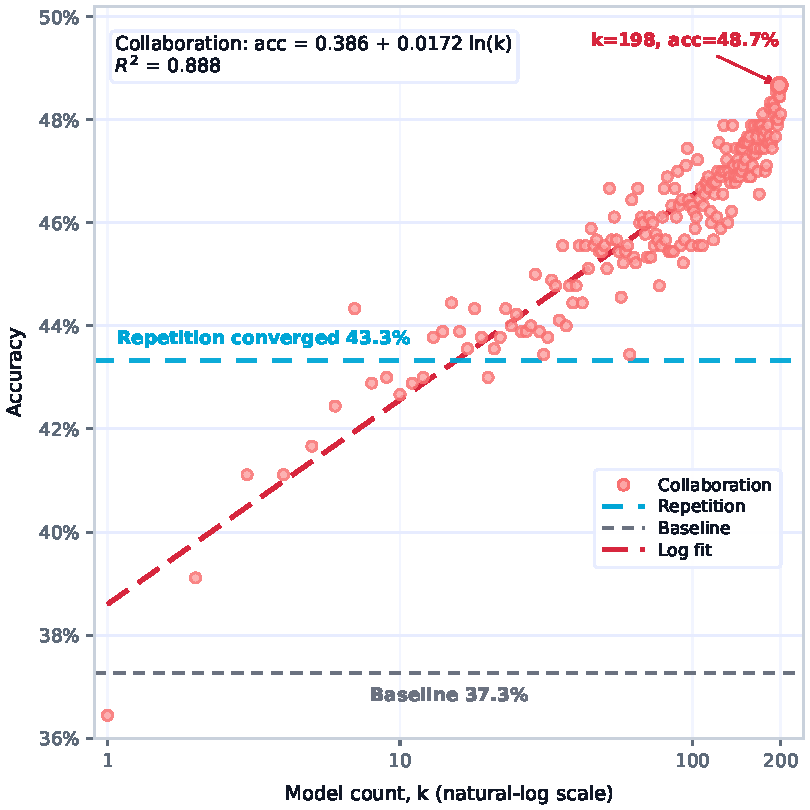
\includegraphics[width=0.52\textwidth]{figures/scale_out/model-count-majority-vote.pdf}
\caption{Model-count scaling by majority vote. Collaboration across distinct LoRA models improves beyond repeated sampling from one model, and the Collaboration curve is approximately linear in $\ln(k)$ over the measured range.}
\label{fig:model-count-majority-vote}
\end{figure}

The main result is shown in \Cref{fig:model-count-majority-vote}: Collaboration improves steadily as \(k\) increases. Accuracy rises from \(0.3644\) at \(k=1\) to \(0.4267\) at \(k=10\), \(0.4633\) at \(k=100\), and a best observed \(0.4867\) at \(k=198\). Relative to the final baseline accuracy of \(0.3727\), the largest gain is about \(+0.1140\). Repetition improves early but saturates sooner, reaching a best accuracy of \(0.4378\) at \(k=24\). At large \(k\), the Collaboration advantage reaches about \(+0.0533\).
Fitting the Collaboration curve against \(\ln(k)\) gives
\begin{equation}
 \mathrm{accuracy} \approx 0.386 + 0.0172 \ln(k),
\end{equation}
with \(R^2 \approx 0.888\) over the observed range. The discovered behavior is not linear in \(k\); it is approximately linear in \(\ln(k)\) (shown in \Cref{fig:model-count-majority-vote}). Adding more collaborating models gives diminishing but predictable returns. We treat this as an empirical law in one controlled regime, not as a universal theorem of model populations. Its importance is that it makes model count a measurable scale-out variable: accuracy can be studied as a function of the number of distinct LoRA-adapted models.

% 非 universal theorem，而是 controlled regime 下的 empirical law。
% \paragraph{An empirical log scaling law.}

% 介绍diversity的好处，为什么性能会更高，而不是噪音
\paragraph{Why diversity is not sampling noise.}

The comparison between Collaboration and Repetition shows that adapter diversity is not equivalent to sampling noise. Repeated sampling from one model helps at small \(k\), because stochastic decoding produces varied answers, but it saturates earlier. Voting across different LoRA instances continues to improve at larger \(k\), suggesting that the population aggregates complementary policies. Importantly, this diversity does not come from unrelated architectures or pretraining corpora. It comes from small PEFT runs following different trajectories under data ordering, masking, stochasticity, and checkpoint timing. Even this modest, cheaply constructed adapter diversity is useful.

% 收尾总结、从一个模型到很多模型，介绍使用lora的好处，再提出future research direction
\paragraph{From one model to a distribution of models.}
Operationally, this experiment would be difficult without PEFT. Training 200 full checkpoints, serving them, extracting answers, and evaluating many random subsets would be expensive and cumbersome. LoRA turns each model into a lightweight variant of the same prior, making controlled population experiments feasible. This is the concrete mechanism behind Scale Out: \textbf{once adapter creation and serving are cheap, researchers can optimize not only a model but a distribution of models.}

The observed log law is not a universal theorem of model populations, but it establishes a research object: accuracy as a function of model count. Future systems may route among adapters, vote across them, cluster them by experience, distill from successful subpopulations, or feed aggregate lessons back into a shared prior. This is why the scale-out thesis emphasizes populations of personal models rather than a single increasingly personalized assistant. Individual adaptation creates value, but populations create a second-order resource: diversity of histories, skills, failures, and successes. The resulting system is not one universal assistant with ever more context, but an ecology of persistent, partially specialized agents.
